\section{Further controls for exposure and competition}
The main calibrated results use a change exclusively to higher-income recommendations. A joint switch for both income groups is a different policy. In the initial 20-block enriched five-listing pilot the lower-income match rate rose from 36.38\% to 45.13\% when only the higher group switched to $T_4$. When both groups switched, the rate was 19.23\%. Endpoint accounting assigns $+10.95$ points to net transfers of occupied listings between income groups and $-2.20$ points to transitions involving vacancies under the higher-only switch. Of 2,790 lower-income instances shown their entire nonempty list, 65 lost a match and 41 gained one. In the ordinary pilot, changing only higher-income lists reduced the lower-income match rate by 0.38 points. These studies share the summer catalogues.

\paragraph{Sensitivity to preferences.}
On the 100 fresh summer blocks, varying the transparent score and the latent renter model together gave the results in Figure~\ref{fig:grid}. At fitted preferences the proportional quota gave lower-income spillovers of $-0.26$ and $-1.33$ points in ordinary and enriched markets. Enriched top-five effects were positive across all nine parameters, while ordinary top-five effects were positive at six and negative at three. The primary and exploratory price-crossing grids used 129,600 DA allocations each on an NVIDIA H200, with complete counts reproduced by an independent sequential implementation. The two grids reuse markets. Primary-grid uncertainty uses 10,000 paired blocks resamples and a simultaneous maximum standardized deviation over 36 contrasts.
\begin{figure}[ht]\centering
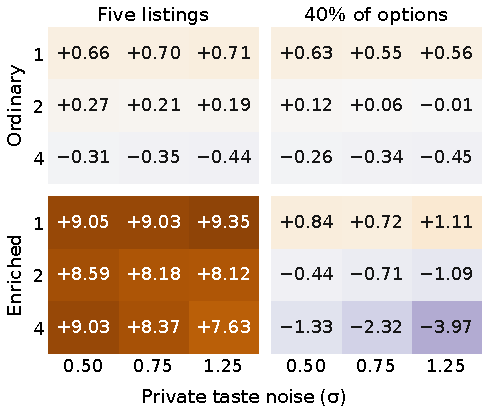
\includegraphics[width=.6\linewidth]{figures/preference_grid.pdf}
\caption{Fresh-block higher-income-only score spillovers (points). Rows within a panel are latent and scoring price weights 1, 2, 4; columns are private taste noise. Ordinary top-five is sensitive to the price assumption.}
\label{fig:grid}\Description{Four three-by-three panels giving signed effects. All enriched top-five cells have positive estimates, while other panels vary.}
\end{figure}

\paragraph{Which part of enrichment matters?}
On 40 further blocks we separately varied the listing draw and the renter-selection rule. Across 408 cell--seed combinations supporting all four arms, the five-listing spillover was $-0.44$ points using ordinary listings and ordinary renters, and $+3.48$ with band listings and the same renters. The paired difference was $+3.92$ ($[3.20,4.70]$). With selected renters these effects were $-0.79$ and $+8.92$. The 72 other ordinary catalogues admitted no eligible lower-income donor for the selected-renter arm. The four-way comparison conditions on common support. The ordinary main comparison includes those scarce markets.

\paragraph{A fixed-quota capacity control.}
Let $\nu(E)$ be full-graph maximum matching cardinality. Among assignments of size $\nu(E)$ choose one with the fewest undisplayed matched pairs; break ties by total observable rank. Its hidden edges are a lower bound on the edits needed to show any such assignment. The bound is attained by replacing each affected renter's worst displayed option with their witness edge, since the witness matches each renter at most once. The rule assumes each renter with eligible options has at least one slot. In the enriched five-listing pilot this changed 11.09\% of slots: visible capacity rose from 24.74 to 55.54 placements per market; DA placements rose from 23.44 to 44.39. The lower-group match rate was 47.58\% against 28.35\% when the same removed slots were randomly replaced, and 36.38\% under uniform lists. Every repaired market still had a full-graph blocker. Archive results include both quotas and market designs.

\paragraph{Verification scope.}
The package includes the summer and winter cohort rules and block-level counts, replay scripts, exact assignments and lower bounds, parameter grids and study designs. The pricing crossover, individual-displacement and stable-quartile analyses are follow-ups to the earlier calibrated results. Different experiments reuse survey households. The winter study evaluates a previously untested scoring intervention on a cohort that had been used for a simpler policy. None of the experiments measures field behavior or validates model-based welfare against outcomes of actual leases.
